\documentclass[a4paper,10pt]{article}

\usepackage[utf8]{inputenc}

\usepackage{hyperref}
\usepackage{graphicx}

% with the default options it reduces the page margins already
\usepackage{geometry}

% glossary {{{
\usepackage[acronym,automake]{glossaries}
\makeglossaries

% \newglossaryentry{WAUT}
% {
%     name=WAUT,
%     description={Web Application Under Test}
% }
\newacronym{waut}{WAUT}{Web Application Under Test}
% }}}

\title{Report: A formal approach for run-time verification of web applications using scope-extended LTL}
\author{Roberto Tonino}

% % cool font {{{
% \usepackage[utf8]{inputenc}
\usepackage{libertine}
% \usepackage{libertinust1math}
% \usepackage[T1]{fontenc}
% % }}}

% biblatex {{{
\usepackage{biblatex}
\addbibresource{report.bib}
% }}}

\usepackage{ifthen}

\newcommand{\tuple}[1]{\mbox{$\langle$#1$\rangle$}}
% \newcommand{\reqmulti}[1]{\mbox{$\langle r_{#1}$,$l_{#1}$,$t_{#1}\rangle$}}
\newcommand{\reqmulti}[1][]{
  \ifthenelse{\equal{#1}{}} {\mbox{$\langle r$,$l$,$t\rangle$}}
  {\mbox{$\langle r_{#1}$,$l_{#1}$,$t_{#1}\rangle$}}
}

\newcommand{\res}[1][]{
  \ifthenelse{\equal{#1}{}}{\mbox{$\langle u$, $c$, $I$, $L$, $V\rangle$}}
  {\mbox{$\langle u_{#1}$, $c_{#1}$, $I_{#1}$, $L_{#1}$, $V_{#1}\rangle$}}
}
\newcommand{\resmulti}[1][]{
  \ifthenelse{\equal{#1}{}}{\mbox{$\langle u$, $c$, $I$, $F$, $L$, $V\rangle$}}
  {\mbox{$\langle u_{#1}$, $c_{#1}$, $I_{#1}$, $F_{#1}$, $L_{#1}$, $V_{#1}\rangle$}}
}



\begin{document}

\maketitle

\tableofcontents

\clearpage

\section{Introduction}
\label{introduction}

In the paper \citetitle{Haydar2013}, the authors propose a model checking approach for formal verification of user defined properties of web applications. The black-box approach was chosen in order to widen the set of web applications that is possible to verify, because it does not require access to source code and is language-agnostic.

The methodology consists in recording traces of a \gls{waut}, converting them in a communicating-automata model, and feeding the model to the model checker Spin. The properties to verify are specified in LTL, which is the property specification language of Spin.

The authors propose a classification of the states of the automata model in \emph{stable}, where all the windows or displays are fully loaded, and \emph{transient} states.  Because of this, it becomes necessary to specify LTL properties over a subset of the states, and beacuse this is tricky even for an expert, the authors propose a LTL operator that allows to specify a LTL formula over subset of states. This operator doesn't affect the expressiveness of LTL, but helps the user in writing more intuitive and succint formulas.

The authors developed a prototype of the proposed approach and in the paper they present the result of using the prototype in a number of web applications.

\section{Automata-based modeling of web applications}
\label{automata-based-modeling-of-web-applications}


\subsection{Modeling approach}
\label{modeling-approach}

The proposed method is not an exaustive testing like traditional model checking, but should be considered as ``passive testing''. Moreover, the authors consider a setting in which the \gls{waut} does not perform asynchronous requests. In other words, the browser is expected to finish loading a page before a subsequent navigation starts.

The monitoring approach proposed contains three main components or modules---\textit{monitoring} module, \textit{analysis} module and \textit{model checking} module. The monitoring module intercepts HTTP requests and responses of the \gls{waut}. The analysis module generates a Promela model taking as input the intercepted traces. Finally, the model checking module verifies user-defined properties against the model generated by the analysis module and produces a counterexample. It uses the Spin model checker.

\subsection{Single window browsing}
\label{single-window-browsing}

This model is a simplified version of the final model, mostly useful to give the reader a gradual introduction to the approach. We now define \emph{web requests}, \emph{responses}, and \emph{browsing sessions}.

\paragraph{Web request}
A \emph{web request} is represented by the string $l$ and can have two shapes:

\begin{enumerate}
  \item if the HTTP method is GET or HEAD, then $l$ is the URI sent in the request;
  \item if the request comes from a form, then $l = a?d$ with
    \begin{itemize}
      \item $a$ form action
      \item $d$ form data, i.e. the key-value fields filled in the form
    \end{itemize}
\end{enumerate}

\paragraph{Response}
A \emph{response} is represented by the tuple \res where:

\begin{itemize}
  \item $u$ represents the request $l$;
  \item $c$ is the status code; $c \in C$ with $C$ set of all status codes (cfr. \cite[\S 15]{Fielding2022});
  \item $I$ is the set of URIs specified by the \textit{action} attribute in all the forms of the page;
  \item $L$ is the set of URIs associated with links. It includes implicit links, but excludes links to document fragments;
  \item $V$ is a vector $\langle$$v_1$, \dots, $v_k$$\rangle$ where $v_i$ is the valuation of the page attribute $i$ and $k$ is the number of all the page attributes over which the atomic propositions are defined.
\end{itemize}

\paragraph{Browsing session}
A \emph{browsing session} is a Request/Response sequence $RRS =$ \res[0] $l_1$ \res[1] \dots $l_n$ \res[n] where:

\begin{itemize}
  \item $u_0$ and $c_0$ are null, and $I_0$, $L_0$, and $V_0$ are empty;
  \item $l_i$ is a request that is followed by the response page \res[i];
  \item for all $i > 1$, $l_i \in L_{i-1}$ if $l_i$ is a request corresponding to a clicked or implicit link;
  \item if $l_i$ is of the form $a_i?d_i$, then $a_i \in I_{i-1}$;
  \item $n$ is the total number of the requests in the browsing session.
\end{itemize}

\paragraph{Attributes}
$\mathcal{U}$ denotes the set of all user-defined attributes.

\subsubsection{Browsing session as automaton}

The authors present an algorithm to convert an $RRS$ into a so-called \emph{session automaton}. A transition in the session automaton represents a navigation via link or via form submission, while a state represents all the pages with equal valuation attributes and set of links ($L$) and form actions ($I$).

Given a browsing session $RRS =$ \res[0] $l_1$ \res[1] \dots $l_n$ \res[n] where $n$ is the total number of observed requests:

\begin{enumerate}
  \item the tuple \res[0] is mapped to a special state called ``inactive'' and denoted $s_0$. In this state, $u_0$ and $c_0$ are null, and $I_0$, $L_0$, and $V_0$ are empty sets;
  \item for all $i > 0$, a tuple \res[i] corresponds to a state of the automaton. Two tuples \res[i] and \res[j] where $j > i$, are mapped to the same state if:
    \begin{itemize}
      \item $c_i = c_j$; 
      \item $I_i = I_j$; 
      \item $L_i = L_j$; 
      \item and $V_i = V_j$. 
    \end{itemize}
    $S$ denotes the set of such states.

  \item to define the alphabet of the automaton, we first define $\Gamma$, $\Delta$ and $Req$:
    \begin{itemize}
      \item $\Gamma = \displaystyle\bigcup_{i=1}^{n} L_i$;
      \item $\Delta \subseteq \displaystyle\bigcup_{i=1}^{n} I_i$;
      \item $Req$ is the set of all observed requests.
    \end{itemize}
    The alphabet is then easily defined $\Sigma = \Gamma \cup \Delta \cup Req$.

  \item a transition is a triple \tuple{$s_i$, $l_{i+1}$, $s_{i+1}$}, where:
    \begin{itemize}
      \item $s_i =$\res[i];
      \item $s_{i+1} =$\res{i+1};
      \item  if $l_{i+1}$ is a request corresponding to a clicked or implicit link, then $l_{i+1} \in L_i$ 
      \item otherwise if $l_{i+1}$ is of the form $a_{i+1}?d_{i+1}$, then $a_{i+1} \in I_i$, and  if $c_{i+1} \neq 3xx$, then $l_{i+1} = u_{i+1}$, otherwise $l_{i+1} \neq u_{i+1}$.
    \end{itemize}

  \item Each request corresponding to an \textbf{explored repeated link} or \textbf{explored repeated form} defines a transition from the state to the state that corresponds to the response of the clicked link or the submitted form.
  \item Each event corresponding to an \textbf{unexplored link} $l \in L_i$ or \textbf{unexplored form} $a \in I_i$ defines a transition from the state representing the page \res[i] to a designated state, called a \emph{trap} state that represents the unexplored part of the WAUT and whose attributes are not available. Let $T$ denote the set of such transitions.
\end{enumerate}

The session automaton is $ARRS = \langle S \cup \{trap\}, s_0, \Sigma, T \rangle$. We define \emph{deduced} states by inferring transitions of links (forms) that are repeated in different pages of the \gls{waut} without being clicked (submitted) in every page where they occur. Deduced states enhance the model obtained by solely considering the traces, increasing the impact of model checking in this setting. Additionally, note that we are merging states which have the same attributes and the same set of outgoing transitions.

\begin{figure}[h]
  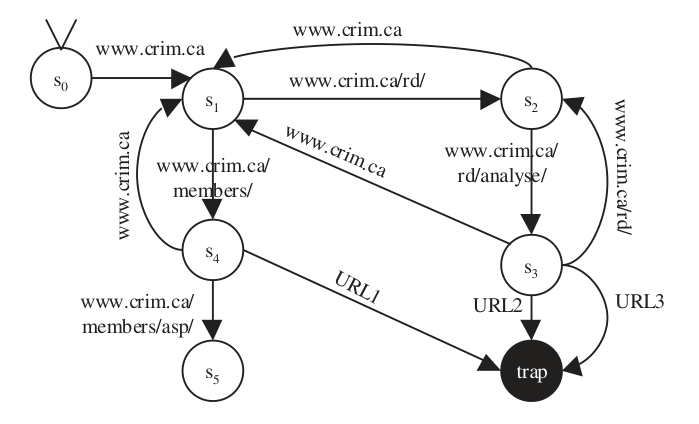
\includegraphics[width=\textwidth]{img/session_automaton_example.png}
  \caption{Example of a session automaton.}
\end{figure}

\subsection{Multiple window browsing}
\label{multiple-window-browsing}

The authors present a model that represents web applications with multiple windows or multiple frames. Such setting introduces concurrency, and increases the number of combination of states in the automaton. The proposed model uses \emph{communicating automata}.

The communicating automata model is a tuple \resmulti. Compared to the previous definition of model automaton, in this setting the sets $I$ and $L$ are extended to include the link targets. Therefore, an element of $L$ is $\langle$$l$, $t$$\rangle$, where $l$ is an URI associated with a link and $t$ is the corresponding target. If no target is defined, $t = \varepsilon$, the empty target. Similarly, an element of $L$ is denoted \tuple{$a$, $t$} with $a$ being a form action attribute. $F$ is the set of frames of the page, with each frame being a tuple \tuple{$f$, $b$}, where $f$ is the URI defined by the value of the \textit{src} attribute of the HTML frame element and $b$ is the frame name.

$RRS$ is a request-response sequence. $RRS = $\resmulti[0]\reqmulti[1]\resmulti[1]\dots\reqmulti[n]\resmulti[n] with $n$ being the total number of requests in the browsing session starting from \reqmulti[1]. \reqmulti[i] represents a request, such that $r_i$ is a string denoting the request header field, ``referer'', which is the URI of the page, where the request was triggered. \tuple{$l_i$,$t_i$} is defined as follows:

\begin{itemize}
  \item if the request is for a filled form, then $l_i$ is of the form $a_i?d_i$, where $a_i$ forms with the target $t_i$ a tuple \tuple{$a_i$,$t_i$} $\in I_j$ of the page \resmulti[j], where $u_j = r_i$;
  \item if the request is for a frame source page, then \tuple{$l_i$,$t_i$} $\in F_j$ of the page \resmulti[j], where $u_j = r_i$;
  \item otherwise (if the request is for a link, clicked or implicit), then \tuple{$l_i$,$t_i$} $\in L_j$ of the page \mbox{\res[j]}, where $u_j = r_i$.
\end{itemize}

As in the case of single window web applications, \resmulti[0] corresponds to the initial default page: 

\begin{itemize}
  \item $u_0$, $c_0$ are null; 
  \item $I_0$, $F_0$, $L_0$, $V_0$ are empty sets;
  \item \reqmulti[1] includes the URI $l_1$ of the starting page;
  \item $r_1$ and $t_1$ are the empty string $\varepsilon$
\end{itemize}

In addition, $l_i = u_i$, if $c_i \neq 3xx$; otherwise $l_i \neq u_i$ and \resmulti[i] immediately follows $r_i$ in the $RRS$. From now on, abbreviations are introduced: \reqmulti is denoted by $R$ and \resmulti is denoted by $P$.

\subsubsection{Communicating automata}

Given a browsing session, first automata on the execution on windows and frames are built, then they are combined in a system of communicating automata. Automata communicate synchronously by executing common (rendezvous) actions. The formal representation of such communication happens with the parallel composition operator on automata.

Formally, two communicating automata $A_1 = $\tuple{$S_1$, $s_{01}$, $\Sigma_1$, $T_1$} and $A_2 = $\tuple{$S_2$, $s_{02}$, $\Sigma_2$, $T_2$} are composed using the \parallel\ operator. The resulting automaton, denoted $A_1\parallel A_2$ is a tuple \tuple{$S$, $s_0$, $\Sigma$, $T$} where 

\begin{itemize}
  \item $s_0 = (s_{01}, s_{02})$ and $s_0 \in S$;
  \item $\Sigma = \Sigma_1 \cup \Sigma_2$;
  \item $S \subseteq S_1 \times S_2$ and $T$ are the smallest sets which satisfy the following rules:
    \begin{itemize}
      \item if $(s_1,e,s'_1) \in T_1$, $e \notin \Sigma_2$, and $(s_1,s_2)\in S$, then $(s'_1,s_2)\in S$ and $((s_1,s_2),e,(s'_1,s_2))\in T$;
      \item if $(s_2,e,s'_2) \in T_2$, $e \notin \Sigma_1$, and $(s_1,s_2)\in S$, then $(s_1,s'_2)\in S$ and $((s_1,s_2),e,(s_1,s'_2))\in T$;
      \item if $(s_1,e,s'_1) \in T_1$, $(s_2,e,s'_2) \in T_2$, and $(s_1,s_2) \in S$, then $(s'_1,s'_2) \in S$, and $((s_1,s_2),e,(s'_1,s'_2)) \in T$.
    \end{itemize}
\end{itemize}

The composition is associative and can be applied to finitely many automata.

\section{Extending the web application model}

\section{LTL and the ``In'' operator}
\label{ltl-and-the-in-operator}

In order to represent more succintly LTL formulas in the domain of web
applications, the authors extend the LTL syntax with the \textbf{In}
operator.

\section{Results}
\label{results}

\clearpage
\printbibliography

\end{document}

% vi: fdm=marker
